%************************************************
\chapter{Experiment 2B: Infra Red Spectroscopy \label{ATR_exp}}
%************************************************
\begin{flushright}
September 13, 2012
\end{flushright}

\section{Objective}
	To study the spectroscopic characteristics of the following compounds using an ATR-FTIR spectroscope.
	\begin{enumerate}
		\item Polymers
		\begin{enumerate}
			\item CD Cover
			\item Teflon		
		\end{enumerate}
		\item Solids
		\begin{enumerate}
			\item Benzaldehyde
			\item Phenol
		\end{enumerate}
		\item Liquids
		\begin{enumerate}
			\item Benzoic Acid
			\item Urea
		\end{enumerate}
	\end{enumerate}

\section{Theory}
	This FTIR part of this section is the same as and has been covered earlier in \autoref{chapter1}. What makes this section special is the word ATR, which stands for Attenuated Total (internal) Reflection. Total internal reflection occurs, as we know, when light travelling in an optically denser medium, is incident on a rarer surface, with an angle greater than some `critical' value, then the light is completely reflected. What has this got to do with spectroscopy, well as it turns out, light when is reflected as aforesaid, it penetrates to about 20 micrometers into the rarer surface. Here's where the fun begins. As the wavelength approaches the absorption range of the rarer substance, the reflected ray undergoes higher attenuation. And that does it! We harness this very property to `scan' through different wavelengths and find the spectrum of the substance.\\
	Experimentally, we use a crystal of a substance of very high refractive index, typically Thallium Bromide/Iodide and let the incident light from the FTIR, enter the crystal as shown in \autoref{2B_atr}, hit the rarer surface multiple times to accumulate attenuation and then allow this light ray to pass through the same FTIR detector. (In our case however, we used $ZnSe$.)\\
	What is the immediate advantage? Aside from the ability to measure spectra of opaque substances, we can use this technique to find spectra of fluids as well. Further, since this is a surface technique, situations where bulk is not of interest, this technique comes to the rescue.

	\begin{figure}[bth]
		\begin{center}
			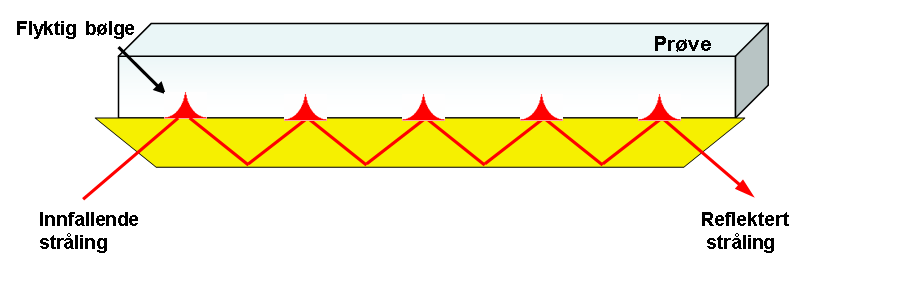
\includegraphics[width=0.8\linewidth]{gfx/02B_atr}
		\end{center}
	\caption[ATR principle]{\label{2B_atr}}
	\end{figure}

\section{Procedure}
	The procedure for ATR is rather straightforward and easily done, unlike the palette preparation requirement in the conventional FTIR.
	\begin{enumerate}
		\item Method for Liquids:
		\begin{enumerate}
			\item Cleaned the $ZnSe$ tray with $CCl_{4}$ and wiped off its excess
			\item Liquid samples were then loaded and the tray covered
		\end{enumerate}
		\item Method for Solids:
		\begin{enumerate}
			\item Powdered the solid finely using Pestle and Mortar and spread evenly on the tray.
			\item The tray was placed and tightened using a screw firmly.
		\end{enumerate}
		\item For Films and Plastics:
		\begin{enumerate}
			\item An extra apparatus provided with the ATR crystal was used.
		\end{enumerate}
	\end{enumerate}

\section{Analysis}
	\begin{enumerate}
		\item CD Cover - \autoref{2B_CD_Cover}
			\begin{table}
				\myfloatalign
				\begin{tabularx}{\textwidth}{Xlll}
					\hline%
					$C-H$ stretching					& 	$2917.68$	& 	$cm^{-1}$\\
					$C-H$ bending						& 	$1376.45$	& 	$cm^{-1}$\\
					\hline%
				\end{tabularx}
				\caption{IR peaks for a CD Cover}
				\label{2B_CD_Cover}
			\end{table}
		\item Teflon - \autoref{2B_Teflon}
			\begin{table}
				\myfloatalign
				\begin{tabularx}{\textwidth}{Xlll}
					\hline%
					$C-F$ stretching					& 	$1206.97$ and $1150.19$ & 	$cm^{-1}$\\
					\hline%
				\end{tabularx}
				\caption{IR peaks for Teflon}
				\label{2B_Teflon}
			\end{table}
		\item Benzaldehyde - \autoref{2B_Benzaldehyde}
			\begin{table}
				\myfloatalign
				\begin{tabularx}{\textwidth}{Xlll}
					\hline%
					$O-H$ due to presence of Benzoic Acid	& 	$3059.5$	& 	$cm^{-1}$\\
					$H-C=O$ stretch						& 	$2738.04$	& 	$cm^{-1}$\\
					Carbonyl $C=O$ stretch					& 	$1583.77$	& 	$cm^{-1}$\\
					\hline%
				\end{tabularx}
				\caption{IR peaks for Benzaldehyde}
				\label{2B_Benzaldehyde}
			\end{table}

		\item Phenol - \autoref{2B_Phenol}
			\begin{table}
				\myfloatalign
				\begin{tabularx}{\textwidth}{Xlll}
					\hline%
					$C-H$ stretch	& 	$3049.49$	& 	$cm^{-1}$\\
					$O-H$ stretch	& 	$3324.03$	& 	$cm^{-1}$\\
					$C-C$ multiple bond stretching	& 	$1450-1600$	& 	$cm^{-1}$\\
					$C-O$ stretching vibration 	& 	$1367.17$	& 	$cm^{-1}$\\
					$O-H$ bending 	& 	$1222.87$	& 	$cm^{-1}$\\
					$C-H$ bending 	& 	$748.40$	& 	$cm^{-1}$\\
					\hline%
				\end{tabularx}
				\caption{IR peaks for Phenol}
				\label{2B_Phenol}
			\end{table}

		\item Benzoic Acid - \autoref{2B_benzoic_acid}
			\begin{table}
				\myfloatalign
				\begin{tabularx}{\textwidth}{Xlll}
					\hline%
					$C-H$ stretch	& 	$2822.7$	& 	$cm^{-1}$\\
					$O-H$ stretch	& 	$2554.7$	& 	$cm^{-1}$\\
					$C=O$ stretch	& 	$1688$	& 	$cm^{-1}$\\
					\hline%
				\end{tabularx}
				\caption{IR peaks for Benzoic Acid}
				\label{2B_benzoic_acid}
			\end{table}

		\item Urea - \autoref{2B_Urea}
			\begin{table}
				\myfloatalign
				\begin{tabularx}{\textwidth}{Xlll}
					\hline%
					$C=O$ stretch	& 	$1598.07$	& 	$cm^{-1}$\\
					$C-N$ stretch	& 	$1460$	& 	$cm^{-1}$\\					
					\hline%
				\end{tabularx}
				\caption{IR peaks for Urea}
				\label{2B_Urea}
			\end{table}

	\end{enumerate}


\section{Reference}
	\begin{enumerate}
		\item Modern Spectroscopy, Fourth Edition, by J. Michael Hollas
		\item \url{http://en.wikipedia.org/wiki/Total_internal_reflection}
		\item Lecture Notes from CHM211 and CHM201, 2012-13
		\item Organic Chemistry by L. G. Wade
	\end{enumerate}

\section{Acknowledgements}
	I acknowledge the contribution of Mr. Arpit Porwal and Ms. Athira Nair, for the performance of the experiment as team members. I specially thank Mr. Arpit Porwal for assisting me with the print outs.\\